%&"../mdl"
\endofdump
\tikzexternalize[prefix=cache/]{hw1}
\begin{document}
    \title{作业一:MLQP}
    \maketitle

    \tableofcontents
    \clearpage

    \section{推导}
    \begin{problem}
        Suppose the output of each neuron in a multi-
layer perceptron is:

\begin{equation}\label{eq:def}
    x_{kj} = f\left(\sum_{i=1}^{N_{k-1}}(u_{kji}x_{k-1,i}^2+v_{kji}x_{k-1,i})+b_{kj}\right)
\end{equation}

where both $u_{kji}$ and $v_{kji}$ are the weights connecting the $i^\text{th}$ unit in the layer $k-1$ to the $j^\text{th}$ unit in the layer $k\in[2,M]$, $b_{kj}$ is 
the bias of the $j^\text{th}$ unit in the layer $k\in[2,M]$, $N_k$ is the number of 
units  if $1\leq k\leq M$ and $f(\cdot)$ is the sigmoidal activation 
function. 

Please derive a back-propagation algorithm for multilayer 
quadratic perceptron (MLQP) in on-line or sequential 
mode.
    \end{problem}

    \begin{figure}[h]
        \centering
        
\includegraphics[height=0.25\textheight]{mlqp}
        \caption{MLQP}\label{fig:mlqp}
    \end{figure}

    \subsection{输出神经元}
        对于输出神经元信号 $x_{Mj}$ 来说,令 $d_{Mj}$ 为目标值,则对应的误差为
        \begin{equation*}
            e_{Mj} = d_{Mj} - x_{Mj}
        \end{equation*}
        % 如果效果不理想,将会采用交叉熵函数。
        使用均方误差计算损失函数
        \begin{equation}\label{eq:loss}
            \mathcal{E} = \sum_{j=1}^{N_{M}}\frac{1}{2}e_{Mj}^2
        \end{equation}
        则对于 $\mathit{net}_{Mj}$ 的梯度为
        \begin{align*}
            \frac{\partial\mathcal{E}}{\partial net_{Mj}} &= \frac{\partial\mathcal{E}}{\partial e_{Mj}}\frac{\partial e_{Mj}}{\partial x_{Mj}}\frac{\partial x_{Mj}}{\partial \mathit{net}_{Mj}} \\
            &= -e_{Mj}f^\prime(\mathit{net}_{Mj})
        \end{align*}
        定义对应的局部梯度(local gradient)为
        \begin{equation}\label{eq:outlocalgrad}
            \delta_{Mj} = -\frac{\partial\mathcal{E}}{\partial net_{Mj}} = e_{Mj}f^\prime(\mathit{net}_{Mj})
        \end{equation}
    \subsection{隐藏层}
    对于隐藏神经元上的 $net_{k-1,j}$ 而言,假设后一层反向传播来的局部梯度已知:
    \begin{equation*}
        \delta_{kj} = -\frac{\partial\mathcal{E}}{\partial\mathit{net}_{kj}}
    \end{equation*}
    则该层的局部梯度为
    \begin{align}
        \delta_{k-1,i} = -\frac{\partial\mathcal{E}}{\partial\mathit{net}_{k-1,i}} &= -\frac{\partial\mathcal{E}}{\partial x_{k-1,i}}\frac{\partial x_{k-1,i}}{\partial\mathit{net}_{k-1,i}} \nonumber\\
        &= -f^\prime(\mathit{net}_{k-1,i})\sum_{j=1}^{N_j}\frac{\partial\mathcal{E}}{\partial\mathit{net}_{kj}}\frac{\partial\mathit{net}_{kj}}{\partial x_{k-1,i}} \nonumber\\
        &= f^\prime(\mathit{net}_{k-1,i})\sum_{j=1}^{N_j}\delta_{kj}(2u_{kji}x_{k-1,i}+v_{kji})\label{eq:hiddenlocalgrad}
    \end{align}
    \subsection{更新权值}
    而根据公式 \eqref{eq:def},
    \begin{align*}
        \frac{\partial\mathit{net}_{kj}}{\partial u_{kji}} &= x_{k-1,i}^2 \\
        \frac{\partial\mathit{net}_{kj}}{\partial v_{kji}} &= x_{k-1,i}
    \end{align*}
    设定学习率分别为 $\eta_1,\eta_2$,则对应权重的修正值
    \begin{align}
        \Delta u_{kji} = -\eta_1\frac{\partial\mathcal{E}}{\partial u_{kji}} 
        &=-\eta_1\frac{\partial\mathcal{E}}{\partial\mathit{net}_{kj}}\frac{\partial\mathit{net}_{kj}}{\partial u_{kji}}=\eta_1\delta_{kj}x_{k-1,i}^2 \label{eq:u}\\
        \Delta v_{kji} = -\eta_2\frac{\partial\mathcal{E}}{\partial v_{kji}} &=-\eta_2\frac{\partial\mathcal{E}}{\partial\mathit{net}_{kj}}\frac{\partial\mathit{net}_{kj}}{\partial v_{kji}}= \eta_2\delta_{kj}x_{k-1,i} \label{eq:v}
    \end{align}
    % 为了提高学习速率,引入动量
    % \begin{align}
    %     \Delta u_{kji}(t+1) &= \alpha_1\Delta u_{kji}(t) + \eta_1\delta_{kj}x_{k-1,i}^2 \\
    %     \Delta v_{kji}(t+1) &= \alpha_2\Delta v_{kji}(t) + \eta_2\delta_{kj}x_{k-1,i} 
    % \end{align}
    % 这里 $\alpha_1$ 和 $\alpha_2$ 分别为其动量常数。
    这个结果与 \cite{MLQP} 基本一致。

    \subsection{更新偏移}

    类似地由于
    \begin{equation*}
        \frac{\partial\mathit{net}_{kj}}{\partial b_{kj}} = 1
    \end{equation*}
    则设定学习率为 $\eta_3$,则对应的偏移修正值
    \begin{equation}\label{eq:bias}
        \Delta b_{kj} = -\eta_3\frac{\partial\mathcal{E}}{\partial b_{kj}}  = -\eta_3\frac{\partial\mathcal{E}}{\partial\mathit{net}_{kj}}\frac{\partial\mathit{net}_{kj}}{\partial b_{kj}} = \eta_3\delta_{kj}
    \end{equation}

    \section{实现}
    \begin{problem}
        Please implement an on-line BP algorithm for MLQP
(you can use any programming language), train an MLQP
with one hidden layer to classify two spirals problem,
and compare the training time and decision boundaries at
three different learning rates.
    \end{problem}

    \subsection{结构设计}

    如图 \ref{fig:network},输入为两个维度上的坐标 $x,y$。采用单输出与硬阈值分类,阈值设定为 0.5,按照 \cite{gate} 的说法,识别时将大于等于 0.5 的设为正类,小于 0.5 的定义为负类,但这并不影响训练过程,因为采用的是原始输出作为误差的计算。
    % 考虑使用 AUC 评估。

    由于只需要一个隐藏层,隐藏层神经元个数为 $N_2$,那么参数个数为
    \begin{equation*}
        2(2N_2+N_2) + N_2 + 1 = 7N_2 + 1
    \end{equation*}
    由于训练集样本数为 300,假设我们想要保持 10\% 的分类错误误差,那么为了好的泛化能力,参数个数应当满足
    \begin{equation*}
        300 = O\left(\frac{7N_2+1}{10\%}\right)
    \end{equation*}
    $N_2$ 至少应当是 5 的倍数级别,仿照 \cite{MLQP},这里取 10。

    \begin{figure}[ht]
        \centering
        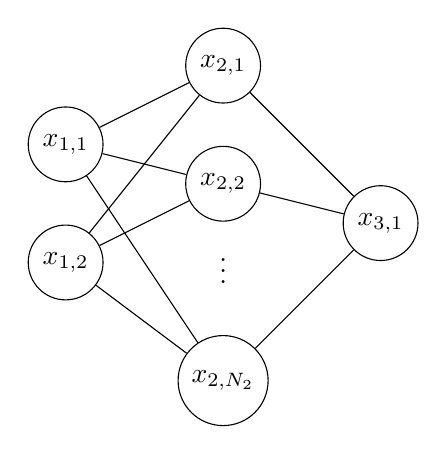
\begin{tikzpicture}
    \tikzstyle{neuron}=[draw,circle];
    \node (x11) [neuron] at (-2,1.5) {$x_{1,1}$};
    \node (x12) [neuron] at (-2,0) {$x_{1,2}$};
    \node [neuron] (x21) at (0,2.5) {$x_{2,1}$};
    \node [neuron] (x22) at (0,1) {$x_{2,2}$};
    \node (x23) [neuron] at (0,-1.5) {$x_{2,N_2}$};
    \node (x31) [neuron] at (2,0.5) {$x_{3,1}$};
    \node at (0,0) {$\vdots$};
    
    \foreach \i in {1,2}{
        \foreach \j in {1,2,3}{
            \draw (x1\i) -- (x2\j);
        }
    }
    
    \foreach \j in {1,2,3}{
        \foreach \k in {1}{
            \draw (x2\j) -- (x3\k);
        }
    }
    
\end{tikzpicture}
        \caption{网络结构}\label{fig:network}
    \end{figure}

    \subsection{算法小结}

    下面将采用矩阵记号简化运算,以下 $\times$ 均表示矩阵的逐点相乘。设第 $k-1$ 层的数值矩阵为 $\mathbf{X}_{k-1}=(x_{k-1,i})_{N_{k-1}\times 1}$,其逐项平方矩阵为 $\mathbf{Y}_{k-1}=(x_{k-1,i}^2)_{N_{k-1}\times 1}=\mathbf{X}_{k-1}\times\mathbf{X}_{k-1}$,向后的权重矩阵为 $\mathbf{U}_{k}=(u_{kji})_{N_{k}\times N_{k-1}}$, $\mathbf{V}_{k}=(v_{kji})_{N_{k}\times N_{k-1}}$,偏移量矩阵 $\mathbf{B}_{k}=(b_{kj})_{N_{k}\times 1}$。

    \subsubsection{前向运算}

    公式 \eqref{eq:def} 将被改写为
    \begin{equation*}
        \mathbf{X}_{k} = f\left(\mathbf{U}_{k}\mathbf{Y}_{k-1} + \mathbf{V}_{k}\mathbf{X}_{k-1} + \mathbf{B}_{k}\right)
    \end{equation*}
    为了简单起见,保留中间结果 
    \begin{align}
        \mathbf{N}_{k}&=\mathbf{U}_{k}\mathbf{Y}_{k-1} + \mathbf{V}_{k}\mathbf{X}_{k-1} + \mathbf{B}_{k}\\
        \mathbf{X}_{k}&=f(\mathbf{N}_k)
    \end{align}

    \subsubsection{后向运算}

    令 $\mathbf{D}_M$ 为目标输出矩阵,将公式 \eqref{eq:outlocalgrad} 改写,输出层的梯度计算为
    \begin{equation}
        \boldsymbol{\delta}_{M} = (\delta_{M,i})_{N_M\times 1} = (\mathbf{D}_M - \mathbf{X}_M)\times f^\prime(\mathbf{N}_M)
    \end{equation}

    改写公式 \eqref{eq:hiddenlocalgrad},隐含层的梯度计算为
    \begin{equation}
        \boldsymbol{\delta}_{k-1} = \left(\mathbf{U}_{k}^T\boldsymbol{\delta}_{k}\times 2\mathbf{X}_{k-1}+\mathbf{V}_{k}^T\boldsymbol{\delta}_{k}\right)\times f^\prime(\mathbf{N}_{k-1})
    \end{equation}

    改写公式 \eqref{eq:u} 和公式 \eqref{eq:v},权重修正矩阵
    \begin{align*}
        \mathbf{\Delta U}_{k} &= (\Delta u_{kji})_{N_{k}\times N_{k-1}} = \eta_1 \boldsymbol{\delta}_k\mathbf{Y}_{k-1}^T \\
        \mathbf{\Delta V}_{k} &= (\Delta v_{kji})_{N_{k}\times N_{k-1}} = \eta_2 \boldsymbol{\delta}_k\mathbf{X}_{k-1}^T 
    \end{align*}

    改写公式 \eqref{eq:bias},偏移修正矩阵
    \begin{equation*}
        \mathbf{\Delta B}_{k} = (\Delta b_{kj})_{N_{k}\times 1} = \eta_3 \boldsymbol{\delta}_{k}
    \end{equation*}

    \subsection{动量项}

    为了加速收敛过程,对修正项添加动量项
    \begin{align}
        \mathbf{\Delta U}_{k}(t+1) &= \alpha_1\mathbf{\Delta U}_{k}(t) + \eta_1 \boldsymbol{\delta}_k\mathbf{Y}_{k-1}^T \\
        \mathbf{\Delta V}_{k}(t+1) &= \alpha_2\mathbf{\Delta V}_{k}(t) + \eta_2 \boldsymbol{\delta}_k\mathbf{X}_{k-1}^T \\
        \mathbf{\Delta B}_{k}(t+1) &= \alpha_3\mathbf{\Delta B}_{k}(t) + \eta_3 \boldsymbol{\delta}_{k}
    \end{align}
    其中 $\alpha_1,\alpha_2,\alpha_3$ 为动量常数。

    \subsection{训练过程}

    \paragraph{参数初始化}

    简便起见,将三个参数的学习率设置为一个相等的值 $\eta_1=\eta_2=\eta_3=\eta$,将动量常数也设为相同的值 $\alpha_1=\alpha_2=\alpha_3=\alpha$。

    类似于 \cite{torchlinear},由于参数数量相对于线性层加倍,将参数初始化为 $\mathcal{U}\left(-\sqrt{\frac{1}{2\times 2}},\sqrt{\frac{1}{2\times 2}}\right)=\mathcal{U}(-0.5,0.5)$ 上的随机值,其中 $\mathcal{U}$ 为一致分布。

    \paragraph{训练}

    数据范围是 $x\in[-6,6],y\in[-6,6]$。训练与验证将采用 3 折交叉验证,测试集只用于测试最终的训练效果。

    \paragraph{早停}

    类似 \cite{tfearly} 中早停机制的实现,将会在最佳验证误差后没有进展的 \texttt{MAX\_EPOCHS}$=200$ 后停止训练,并恢复最佳模型。

    可以设定一个训练轮次阈值来防止无限训练。
    
    % TODO: talk about the code process.

    \subsection{实验结果}

    为公平起见,防止偶然性,对 $\eta=0.01,0.05,0.1$ 三个学习率,将动量常数固定为 $\alpha=0.8$,都用同样的一组随机种子取平均得到其对应的平均训练时间以及平均测试误差,结果如表 \ref{tab:benchmark_lr} 所示。由表可见,$\eta=0.05$ 综合表现最好。

    \begin{table}[H]
        \centering
        \caption{不同学习率训练时间}\label{tab:benchmark_lr}
        \begin{tabular}{crrr}
            \toprule
            $\eta$ & 0.01 & 0.05 & 0.1 \\
            \midrule
            平均训练时间(s) & 108 & 71 & 32 \\
            平均测试误差(MSE) & 0.1227 & 0.1188 & 0.1303 \\
            \bottomrule
        \end{tabular}
    \end{table}

    都采用 42 随机种子,可视化边界结果如图 \ref{fig:benchmark_lr} 所示,图的下方为训练集误差、验证集误差、监测测试误差对于不同轮的趋势图。

    \begin{figure}[H]
        \centering
        
\includegraphics[width=\linewidth]{benchmark_lr}
        \caption{不同学习率测试结果(随机种子 42)}\label{fig:benchmark_lr}
    \end{figure}

    \section{最小最大模块网络}

    \begin{problem}
        This section will construct a min-max modular network.
        \begin{enumerate}
            \item Divide the two spirals problem into four or nine sub-problems randomly and with prior knowledge, respectively.
            \item Train MLQP on these sub-problems and construct two min-max modular networks.
            \item Compare training time and decision boundaries of the above two min-max modular networks.
        \end{enumerate}
    \end{problem}

    \subsection{分解子问题}

    根据 \cite{minmax},对于子问题有两个原则。
    \begin{lemma}[最小化原则]\label{lemma:min}
        训练集具有相等正类集合的模块应当进行最小化合并。
    \end{lemma}
    \begin{lemma}[最大化原则]\label{lemma:max}
        训练集具有相等负类集合的模块应当进行最大化合并。
    \end{lemma}

    % 由于实验电脑有 4 个逻辑核以及为了简便起见,这里将问题分解为 4 个子问题。
    分解方法是将训练集按照正类集合 $P$ 和负类集合 $N$ 分割,然后将正类集合随机平分为 $k$ 份$P_1,P_2,\cdots,P_k$,负类集合也同样分为 $N_1,N_2,\cdots,N_k$,之后从正类小集和负类小集里分别取一个组合成新的训练集
    \begin{equation*}
        C_{ij} = (P_i, N_j)\quad \forall i,j\in\mathbb{N}\cap[1,k]
    \end{equation*}

    \subsection{构造最小最大模块网络}

    % 如图 \ref{fig:minmax} 所示,可以通过更改合并节点的顺序来构造两个网络:先最小化合并,再最大化合并;先最大化合并,再最小化合并。按照上述引理 \ref{lemma:min} 和 \ref{lemma:max} 的原则,安排节点的合并顺序。

    如图 \ref{fig:minmax} 所示,MIN 节点负责将同正类集的结果合并,MAX 节点负责将同负类集的节点合并。需要合并 $k^2$ 个训练单元的结果。

    \begin{figure}[H]
        \centering
        \providecommand{\minmax}[1]{
	\begin{tikzpicture}[every node/.style={scale=0.6},scale=0.6]
	\tikzstyle{compute}=[draw,circle];
	\tikzstyle{merger}=[draw,rectangle,minimum width=1.5cm,minimum height=1cm];
	\def\k{#1}

	\node [merger] (Max) at (5,-{(\k+1)*(\k+1)}) {MAX};
	\foreach \x in {1,...,\k}{
		\node [merger] (M\x) at (2,{-(2*\x*\k+\k+1)}) {MIN};
		\foreach \y in {1,...,\k}{
			\node [compute] (C\x\y) at (-1, -{2*(\x*\k+\y)}) {$(P_\x,N_\y)$};
			\node [left of=C\x\y,xshift=-1cm] (Cn\x\y) {$C_{\x,\y}$};
			\draw (Cn\x\y) edge (C\x\y);
			\draw (C\x\y) -| (M\x);
		}
		\node [merger,fill=white] at (2,{-(2*\x*\k+\k+1)}) {MIN}; % dummy
		\draw (M\x) -| (Max);
	}
	\node [merger,fill=white] at (5,-{(\k+1)*(\k+1)}) {MAX}; %dummy

	\node [right of=Max,xshift=1cm] (O) {$O$};
	\draw (Max) -- (O);
	\end{tikzpicture}
}
        \subfigure[4 个子问题]{\minmax{2}}
        \subfigure[9 个子问题]{\minmax{3}}
        \caption{网络结构}\label{fig:minmax}
    \end{figure}

    % \subsection{训练过程}

    % TODO: 并行实现

    \subsection{测试结果}

    对于两种情况,采用同一组随机种子进行测试,固定 $\eta=0.05, \alpha=0.8$,测试结果取平均如表 \ref{tab:minmax} 所示。结果显示,随着 $k$ 的增大,每个训练集上的训练时间会减少(由于训练集的体量小,早停比较快),但是总体测试误差会增大。对于随机种子 42 的网络结果可视化结果如图 \ref{fig:boundary_minmax} 所示。

    \begin{table}[H]
        \centering
        \caption{最大最小模块网络测试结果}\label{tab:minmax}
        \begin{tabular}{crr}
            \toprule
            $k$ & 2 & 3 \\
            \midrule
            平均最大时间(s) & 118 & 66 \\
            平均测试误差(MSE) & 0.1339 & 0.1459 \\
            \bottomrule
        \end{tabular}
    \end{table}

    \begin{figure}[H]
        \centering
        \subfigure[4 个子问题]{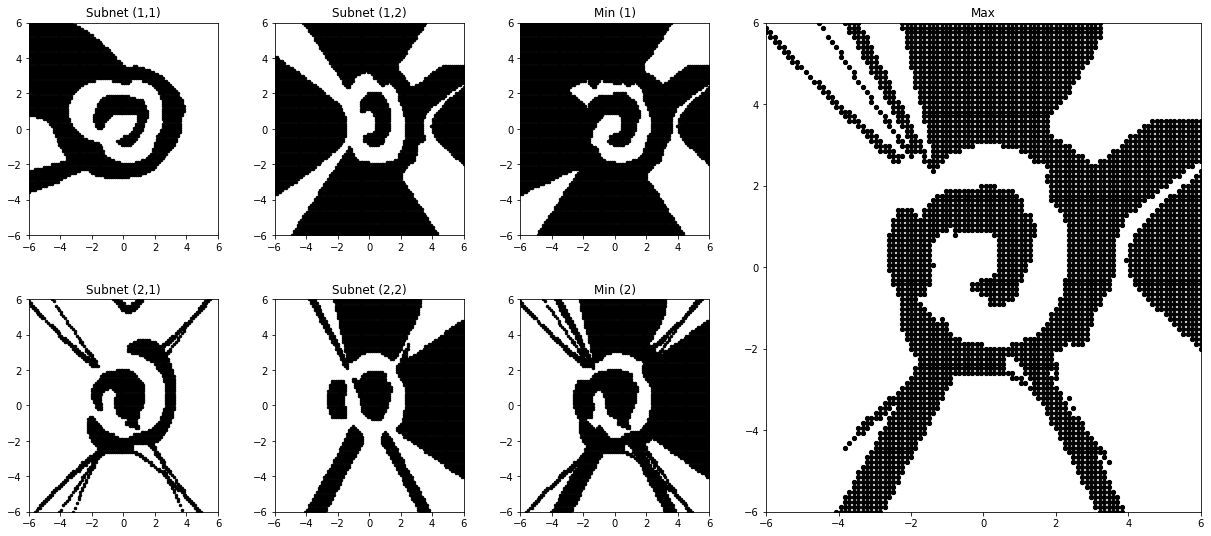
\includegraphics[width=\linewidth]{boundary_minmax2}}
        \subfigure[9 个子问题]{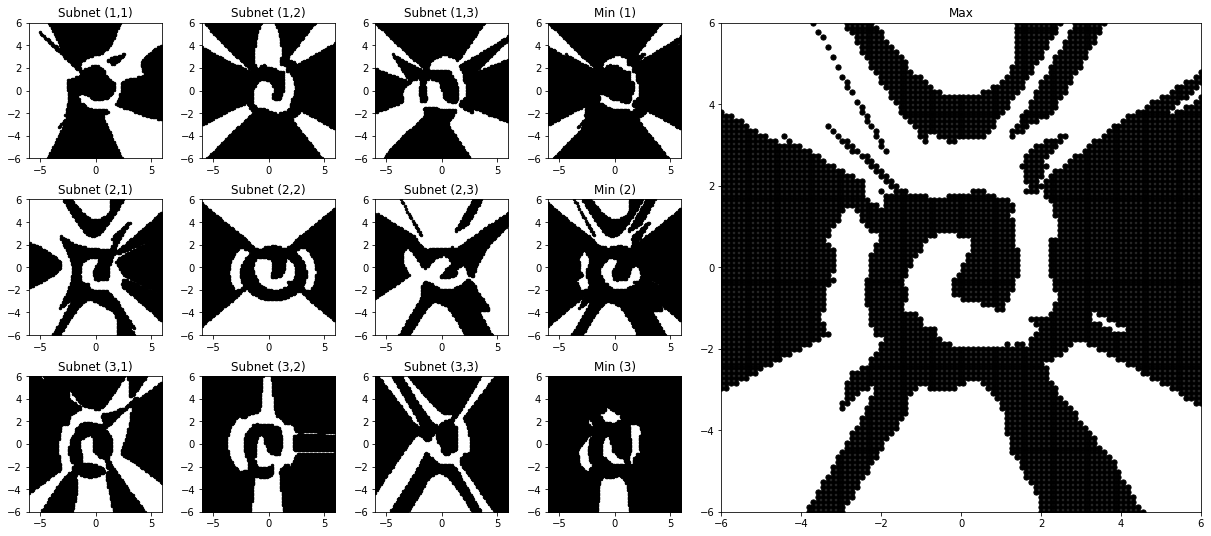
\includegraphics[width=\linewidth]{boundary_minmax3}}
        \caption{最小最大模块网络测试结果(随机种子 42)}\label{fig:boundary_minmax}
    \end{figure}

    \bibliography{ref}

    \appendix

    \section{运行方法}

    所有的代码文件放在 src 文件夹中。运行程序前需要进入 \texttt{src} 目录。
    
    \begin{figure}[H]
        \centering
        \begin{tikzpicture}
    \tikzstyle{folder}=[draw,font=\ttfamily,right];
    \tikzstyle{file}=[draw,font=\ttfamily,right];
    \node [folder] (f) at (-0.5,0.5) {\faFolder{} src};
    \node [file] (f1) at (0.5,-0.5) {\faFile{} minmax.py};
    \node [right] at (5,-0.5) {MIN-MAX 模块网络};
    \node [file] (f2) at (0.5,-1.5) {\faFile{} model.py};
    \node [right] at (5,-1.5) {MLQP 模型};
    \node [file] (f3) at (0.5,-2.5) {\faFile{} util.py};
    \node [right] at (5,-2.5) {实用函数};
    \node [file] (f4) at (0.5,-3.5) {\faFile{} visual.ipynb};
    \node [right] at (5,-3.5) {可视化笔记本};
    \draw  (f) |- (f1);
    \draw (f) |- (f2);
    \draw (f) |- (f3);
    \draw (f) |- (f4);
\end{tikzpicture}
        \caption{源文件目录结构}\label{fig:files}
    \end{figure}

    \subsection{MLQP 模型}
    运行 \filelink{src/model.py}。

    \begin{lstlisting}[style=commandshell]
python model.py [-h] [--epochs N] [--train_file TR] [--test_file TE] [--lr LR] [--alpha A]

optional arguments:
  -h, --help       show this help message and exit
  --epochs N       number of epochs to train (default: 100)
  --train_file TR  training data file
  --test_file TE   test data file
  --lr LR          learning rate (default: 0.1)
  --alpha A        Momentum constant (default: 0.8)
    \end{lstlisting}

    可以设定训练轮次阈值、训练文件、测试文件、学习率以及动量常数。均具有默认参数。

    \subsection{MIN-MAX 模块网络}
    运行 \filelink{src/minmax.py}。

    \begin{lstlisting}[style=commandshell]
python minmax.py [-h] [--k K] [--epochs N] [--lr LR] [--train_file TR] [--test_file TE]

optional arguments:
  -h, --help       show this help message and exit
  --k K            number of split to train (default: 3)
  --epochs N       number of epochs to train (default: 100)
  --lr LR          learning rate (default: 0.1)
  --train_file TR  training data file
  --test_file TE   test data file
    \end{lstlisting}

    可以设定分割份数、训练轮次阈值、学习率、训练文件、测试文件。均具有默认参数。

    \subsection{结果可视化}

    打开 \filelink{src/visual.ipynb} 可以看到普通 MLQP 和 MIN-MAX 网络测试可视结果。调用更加底层的函数时可以设定随机种子。
\end{document}